\section{Introduction}
Our Task in this intership was to find a machine learning method to control a robot arm such that robot arm throw a object in form of a cylinder as far as possible from his original position. For this expiremental task we got a Gazebo environment with a Table, a Hollie robot arm who was fixed on the table, a cylinder to throw and a camera which points on the cylinder, see Fig. \ref{init_state}.
As the focus in this intership was in neurorobotics we chose to use spiking neural network(SNN) as machine learning method. The goal was now to find a suitable learning algorithm for a spiking neuronal network which could solve the task. We came to the conclusion that a reinforcment learning algorithm was the best way to let the network learn and after search of reinforcment algorithms we diced to use evolutional Algorithms. 
To design a spiking neuronal network we used the neurorobotic platform. It's a platform specialized for develop and train spiking neuronal networks. For that the platform includes the following things:
 \begin{itemize}
\item a Gazebo environment and simulation
\item editors to create transfer functions to control the actors and get sensor data
\item a editor to create the neurons and synapsis of the network
\item a view output mechanism to monitor the simulation
\item a so called virtual coach configure and start simulations for the learning task.
\end{itemize} 
\begin{figure}[H]
	\centering
	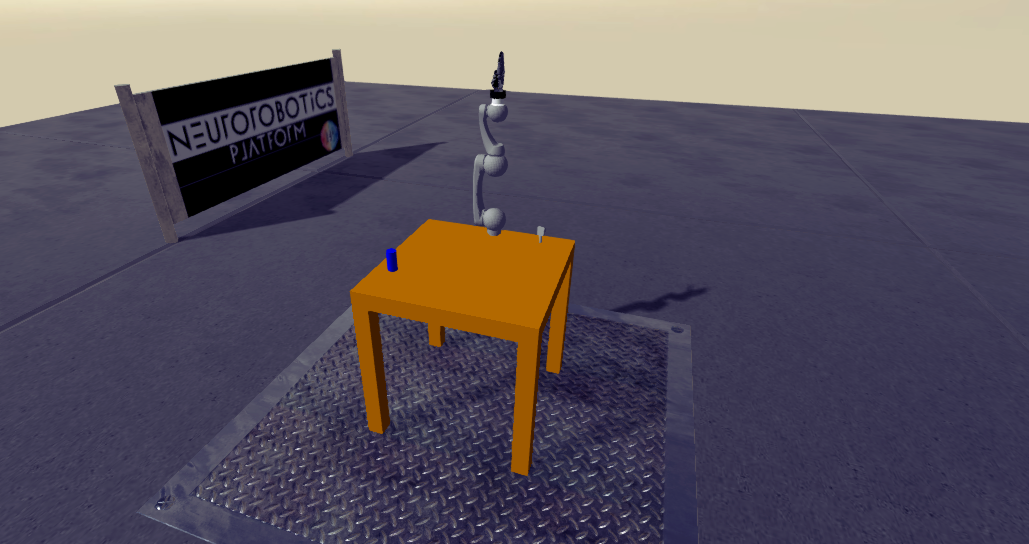
\includegraphics[width=2.2in]{img/init_state.png}
	\DeclareGraphicsExtensions.
	\caption{General task enviornment with inital state }
	\label{init_state}
\end{figure}
\section{Related Work}
As we use Reinforcment Learning and spiking neuronal networks we do here a short instruction to them.
\subsection{Reinforcment Learning}
Reinforcment Learning is based on the interaction of a agent (in our case the robot arm) with his environment (in our case Gazebo). To Learn, the agent get for every action in a state a reward(distance) - depending on if the action was good or not(far or short distance)- and a new state. If the action in the corresponded state got a high reward, then it's more likeliky that the actor uses the same action next time he is in this state again. To see a simple illustration of the whole learning process see Fig. \ref{re_base}
\begin{figure}[H]
	\centering
	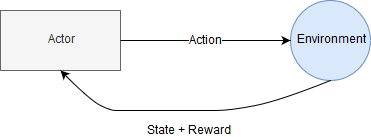
\includegraphics[width=2.2in]{img/re_base.png}
	\DeclareGraphicsExtensions.
	\caption{General illustration of reinforcement learning}
	\label{re_base}
\end{figure}

\subsection{Spiking Neuronal Networks}
Spiking neuronal networks is a variant of artifical neuronal(ANN) networks which are closer to the human brain as model then other ANN. In SNN the information isn't represented by the autoput value of a neuron, as spikes of a single neuron always looks the same, it's represented in the timing a neuron spikes. For example the information can be represented by the difference from the present spike to the last spike. To learn, there are, as in other ANN's weights which describes how much a output spike of a previous neuron influence the next neuron in order. To train the SNN u have to adept this weights, which is quiet difficult as there is no activation function like in standard ANNs. Compared to other ANNs in SNNs each neuron got a activation potential and every time this got exceeded the neuron spikes with a predefined spike.

\section{Throwing Challenge}
\subsection{Task}
As said our Task in this intership was to throw a cylinder as far as possible form a table. For this the experiment we got the following sequenz of events.
 \begin{itemize}
\item State 1 inital state: The robot arm and the cylinder are in their original state, see Fig. \ref{init_state}.
\item State 2 throwing state: The robot arm move to the cylinder to throw or bump him away as far as possible. If the cylinder lands on the ground or 20 sec are over go back to state 1.
\end{itemize}
Our goal was now to optimaze the robot moves in state 2 with a SNN. For that we had to control 7 parameters with a SNN, 6 for the angles of the robot arm + 1 for open and close the hand. 
To achieve the goal we diceded to devide our taks in 3 smaller Task:
 \begin{itemize}
\item 1. Approach the Cylinder
\item 2. Grap the Cylinder
\item 3. Throw the Cylinder
\end{itemize}
In the End of our intership the task 1 and 2 were hard coded and task 3 was achieved with a SNN.
\subsection{Challenges}
\label{challenges}
While the intership we encountered with a view problemms. The most important were:
 \begin{itemize}
\item The Gazebo simulation got a non determensitic bahaviour so it was hard to find good weights for the SNN, as it was hard to reporoduce the same behaviour with the same weights
\item Gripping the Cylinder with the hand. Trough non determenistic behaviour of the simulation it was possible that sometimes the hand didnt crapped the cylinder although it crapped the cylinder many times before with the same joint configuration. This could led to unaccurate results in training, as our precodition in training was that the robot crapped the cylinder.
\item Exploding hand, sometimes the hand just exploding and the cylinder buged away this lead to unrealistic high distances.
\item The Distance measurement wasn't realy acurate, sometimes we a achieved big distance with small throws.
\end{itemize}


